\documentclass[11pt]{article}
\usepackage[margin=2.6cm]{geometry}
\usepackage{amsmath,amssymb,amsthm}
\usepackage{booktabs}
\usepackage{array}
\usepackage{tikz}
\usetikzlibrary{arrows.meta}
\usepackage[colorlinks=true,linkcolor=blue!45!black,citecolor=blue!45!black,urlcolor=blue!45!black]{hyperref}

\newtheorem{theorem}{Theorem}[section]
\newtheorem{lemma}[theorem]{Lemma}
\newtheorem{corollary}[theorem]{Corollary}
\theoremstyle{definition}
\newtheorem{definition}[theorem]{Definition}
\newtheorem{remark}[theorem]{Remark}
\newtheorem{example}[theorem]{Example}

\newcommand{\Zw}{\mathbb{Z}[\omega]}
\newcommand{\Z}{\mathbb{Z}}
\newcommand{\Q}{\mathbb{Q}}
\newcommand{\R}{\mathbb{R}}
\newcommand{\C}{\mathbb{C}}
\newcommand{\Lam}{\Lambda}
\newcommand{\Lmax}{\Lambda_{\max}}
\newcommand{\Gmin}{G_{\min}}
\newcommand{\rep}{\operatorname{rep}}
\newcommand{\N}{\mathsf{N}}
\newcommand{\HNF}{\operatorname{HNF}}
\newcommand{\word}{w}

\title{A canonical form for integer symbols of periodic tilings\\ by regular polygons}
\author{TilingAtlas working note\thanks{Reference implementation and the full adversarial
verification record (differential oracle, attack suites, corpora) accompany this note in
\texttt{docs/canonical-form/verification/}.}}
\date{July 9, 2026}

\begin{document}
\maketitle

\begin{abstract}
Soto S\'anchez, Weyrich, Medeiros e S\'a and de Figueiredo encode an edge-to-edge periodic
tiling of the plane by unit-edge regular polygons as a $(2+n)\times 4$ integer matrix over
$\Z[\omega]$, $\omega=e^{2\pi i/12}$: two rows span a period lattice, the remaining $n$ rows
list one vertex per translation class. One tiling has infinitely many symbols. We define a
computable canonical form $\N$ and prove it sound and canonical for the equivalence
$V'=gV+c$ with $g$ in the dihedral group $D_{12}$ and $c\in\Zw$. The lattice-basis,
seed-representative and seed-order ambiguities are eliminated by construction (Hermite
normal form, canonical coset representatives, row sorting); the $24n$-fold frame ambiguity
(orientation and origin) is cut to the stabilizer of an intrinsic invariant, the multiset of
vertex stars, and the residual minimization is proved to compare byte-identical candidates
whenever its ties come from symmetries of the tiling. Along the way we exhibit a defect in
the naive symbol equivalence: the four commonly listed ambiguity sources do not generate
equivalence of vertex sets, because a tiling can be re-encoded over any finite-index
sublattice of its period lattice; a correct canonical form must therefore recompute the
maximal translation lattice, and ours does. We give complexity bounds, run the form on the
required worked instances, and report an adversarial verification campaign in which no
counterexample to canonicity was found.
\end{abstract}

\section{Setting}\label{sec:setting}

Let $\omega=e^{2\pi i/12}$, with minimal polynomial $\Phi_{12}(x)=x^4-x^2+1$, so
$\omega^4=\omega^2-1$. The ring $\Zw$ is a free $\Z$-module with basis
$(1,\omega,\omega^2,\omega^3)$; we identify $p\in\Zw$ with its coordinate row vector in
$\Z^4$. Multiplication by $\omega$ and complex conjugation are $\Z$-linear maps preserving
$\Zw$. Following~\cite{soto2021integer}, an edge-to-edge periodic tiling by unit-edge
regular polygons, normalized so that one vertex is $0$ and all edges point along
$\omega^0,\dots,\omega^{11}$ (this excludes exactly the octagon-bearing truncated square
tiling, whose edges lie off the $30^\circ$ grid), is recorded by its vertex set
$V\subset\Zw$: choosing a rank-2 period lattice $\Lam=\Z t_1+\Z t_2$ with
$t_1,t_2$ $\R$-linearly independent in $\C$ and $V+\Lam=V$, the set $V$ is a finite union
of cosets
\[
  V=\bigcup_{s\in S}(s+\Lam),\qquad S\subset\Zw/\Lam,\ |S|=n,\ 0\in S ,
\]
and the \emph{symbol} is the $(2+n)\times4$ integer matrix $M$ with rows
$t_1,t_2,s_1,\dots,s_n$. Edges are recovered by joining $v$ to $v+\omega^k$ whenever both
are vertices; the polygons are implicit.

Two vertex sets represent the same tiling exactly when
\begin{equation}\label{eq:equiv}
  V' \;=\; gV+c,\qquad g\in G,\ c\in\Zw,
\end{equation}
where $G=\{\rho_j\colon z\mapsto\omega^j z\}\cup\{\mu_j\colon z\mapsto\omega^j\bar z\}$ is
the dihedral group $D_{12}$ of order 24, acting by integer matrices on $\Z^4$. We write
$M\sim M'$ when the vertex sets of two symbols satisfy~\eqref{eq:equiv}. A \emph{canonical
form} is a computable map $\N$ on symbols with $\N(M)\sim M$ (soundness) and
$M\sim M'\Rightarrow \N(M)=\N(M')$ as integer matrices (canonicity).

The classical inventory of symbol ambiguities lists four sources: (1) the lattice basis,
$U\in GL_2(\Z)$; (2) each seed representative, mod $\Lam$; (3) the seed order; (4) the frame,
i.e.\ origin ($n$ choices) and orientation ($g\in G$, 24 choices). Source~4 is the
substantial one; a brute-force baseline canonicalizes by minimizing over all $24n$ frames.
Section~\ref{sec:stagea} shows this list is incomplete as a generating set
for~\eqref{eq:equiv}.

\section{Preliminaries}\label{sec:prelim}

\begin{lemma}[Hermite normal form, rank 2 in $\Z^4$]\label{lem:hnf}
Every rank-2 sublattice $\Lam\subset\Z^4$ has a unique basis $(h_1,h_2)$ such that, writing
$c_i$ for the position of the first nonzero entry of $h_i$ and $p_i=h_i[c_i]$: $c_1<c_2$,
$p_1,p_2>0$, and $0\le h_1[c_2]<p_2$. Uniqueness includes the entries outside the pivot
columns $c_1,c_2$.
\end{lemma}

\begin{proof}
Let $c_1$ be the first coordinate not identically zero on $\Lam$ and $p_1>0$ the generator
of the image of the projection $\pi_{c_1}\colon\Lam\to\Z$. The kernel
$\Lam_2=\{v\in\Lam: v[c_1]=0\}$ satisfies $\Lam/\Lam_2\cong\Z$, so it has rank 1 and a
unique generator $h_2$ whose first nonzero entry $p_2:=h_2[c_2]$ is positive; its pivot
$c_2$ exceeds $c_1$ because all of $\Lam$ vanishes on coordinates before $c_1$. Pick
$u\in\Lam$ with
$u[c_1]=p_1$ and set $h_1=u-\lfloor u[c_2]/p_2\rfloor h_2$; any two candidates differ by an
element of $\Lam_2=\Z h_2$ whose $c_2$-entry lies in $(-p_2,p_2)$, hence by $0$. Both $h_1$
and $h_2$ are thereby pinned as vectors, free columns included. See
also~\cite[\S2.4]{cohen1993} for the general theory.
\end{proof}

\begin{definition}[canonical coset representative]\label{def:rep}
For $\Lam$ with HNF basis $(h_1,h_2)$ as above and $v\in\Z^4$, let $\rep_\Lam(v)$ be the
unique element $r\in v+\Lam$ with $r[c_1]\in[0,p_1)$ and $r[c_2]\in[0,p_2)$, computed by two
floor divisions (reduce by $h_1$, then by $h_2$; the second step does not disturb
coordinate $c_1$ since $h_2[c_1]=0$).
\end{definition}

Uniqueness: a difference $ah_1+bh_2$ with both pivot coordinates in the open box forces
$|a|p_1<p_1$, so $a=0$, then $b=0$. In particular $\rep_\Lam$ depends only on the coset and
on $\Lam$ itself, not on any basis, and $\rep_\Lam(0)=0$.

\begin{lemma}[direction covariance]\label{lem:sigma}
For $g\in G$ define $\sigma_g\in\mathrm{Sym}(\Z/12)$ by $\sigma_{\rho_j}(k)=j+k$ and
$\sigma_{\mu_j}(k)=j-k$. Then $g(v+\omega^k)=g(v)+\omega^{\sigma_g(k)}$ for all
$v\in\Zw$, and $g\mapsto\sigma_g$ is a group homomorphism.
\end{lemma}

\begin{proof}
$g$ is $\Z$-linear and $g(\omega^k)$ equals $\omega^{j+k}$ for $g=\rho_j$ and
$\omega^{j}\overline{\omega^{k}}=\omega^{j-k}$ for $g=\mu_j$. The homomorphism property
follows from $(g_1g_2)(\omega^k)=g_1(\omega^{\sigma_{g_2}(k)})
=\omega^{\sigma_{g_1}\sigma_{g_2}(k)}$.
\end{proof}

\section{Normalizing the lattice, and a defect in the four-source list}\label{sec:stagea}

For a vertex set $V$ let $\Lmax(V)=\{t\in\Zw: t+V=V\}$, the full translation lattice.

\begin{lemma}[Stage A]\label{lem:stagea}
Let $(\Lam,S)$ encode $V$ with $S=\{s_1,\dots,s_n\}\subset\Zw/\Lam$, and let
$T=\{\tau\in\Zw/\Lam : S+\tau=S\}$. Then:
\begin{enumerate}\itemsep2pt
\item[(a)] $T$ is a subgroup of $\Zw/\Lam$ and $\Lmax(V)$ is its full preimage in $\Zw$;
  in particular $\Lam\subseteq\Lmax(V)$.
\item[(b)] Every $\tau\in T$ occurs among the $n$ candidates $s_j-s_1$, $j=1,\dots,n$.
\item[(c)] For a candidate $\tau$, the inclusion $S+\tau\subseteq S$ already implies
  $S+\tau=S$.
\item[(d)] Every $\tau\in T$ has finite order in $\Zw/\Lam$; hence the lattice generated by
  $\Lam$ and lifts of $T$ has rank 2 and equals $\Lmax(V)$.
\item[(e)] $\Lmax(hV+c)=h\,\Lmax(V)$ for all $h\in G$, $c\in\Zw$.
\end{enumerate}
\end{lemma}

\begin{proof}
(a) $t+V=V$ iff $(S+t)+\Lam=S+\Lam$ iff $S+(t\bmod\Lam)=S$. (b) $\tau+s_1\in S$, so
$\tau\equiv s_j-s_1$ for some $j$. (c) Adding $\tau$ is injective on $\Zw/\Lam$ and $S$ is
finite, so an injection of $S$ into itself is a bijection. (d) The orbit
$\{s_1+m\tau\}_{m\ge0}$ lies in the finite set $S$, so $m\tau=m'\tau$ for some $m>m'$ and
$(m-m')\tau=0$; thus $\Lmax\otimes\Q=\Lam\otimes\Q$ has rank 2, and $\Lmax$ is generated by
$\Lam$ together with the finitely many elements of $T$, all of which appear in (b).
(e) $t+hV+c=hV+c$ iff $h^{-1}t+V=V$.
\end{proof}

Stage A of our algorithm computes $\Lmax$ by Lemma~\ref{lem:stagea}: test the $n$
candidates, stack the valid ones on $\Lam$, take the HNF (Lemma~\ref{lem:hnf}), reduce all
seeds by $\rep_{\Lmax}$ and remove duplicates. The result $(\Lmax,S)$ depends only on $V$.

\begin{remark}[the defect]\label{rem:gap}
The four ambiguity sources of Section~\ref{sec:setting} all preserve $n$, but
equivalence~\eqref{eq:equiv} does not: the encoding definition requires only \emph{some}
invariant rank-2 lattice, so the same $V$ admits a symbol over every finite-index sublattice
$\Lam'\subset\Lmax(V)$, with $n\cdot[\Lmax:\Lam']$ seeds. Concretely, the square tiling
$V=\Z+\Z i$ has the $n{=}1$ symbol of Example~\ref{ex:square} and also an $n{=}4$ symbol
over $2\Z+2\Z i$; the two vertex sets are literally equal, hence equivalent
under~\eqref{eq:equiv}. A baseline that canonicalizes the \emph{given} lattice by HNF and
minimizes over $24n$ frames assigns these two symbols matrices of different shapes, so it
is not canonical for~\eqref{eq:equiv}; we verified this computationally on a faithful
implementation. Any correct $\N$ must therefore recompute $\Lmax$, as Stage A does.
Alternatively one may read lattice maximality as an unstated precondition on valid symbols;
then Stage A is input validation rather than a correction, and it certifies the
precondition at the same cost. Whether the convention of~\cite{soto2021integer} already
requires maximality should be checked before attributing the defect beyond the problem
statement we received; in an enumeration pipeline the point is moot, since period-solving
stages do not in general certify maximal periods, and a dedup key without Stage A can leak
duplicates either way.
\end{remark}

\section{Stars and the frame rule}\label{sec:stars}

\begin{definition}[stars, words, frame invariants]\label{def:star}
For a vertex class $[s]\in V/\Lmax$ let
$\mathrm{star}(s)=\{k\in\Z/12 : s+\omega^k\in V\}$, computed as
$\{k:\rep_{\Lmax}(s+\omega^k)\in S\}$. Encode subsets $A\subseteq\Z/12$ as words
$\word(A)=\sum_{k\in A}2^{11-k}$. For $g\in G$ let $L_g(V)$ be the ascending list of the
$n$ words $\word(\sigma_g(\mathrm{star}(s)))$, $[s]\in V/\Lmax$. Define
\begin{gather*}
  \Gmin(V)=\operatorname*{arg\,min}_{g\in G} L_g(V)
  \quad(\text{lexicographic order on lists}),\\
  A_g(V)=\{[o] : \word(\sigma_g(\mathrm{star}(o)))=\min L_g(V)\}.
\end{gather*}
Elements of $A_g$ are the \emph{anchors} (candidate origins) for orientation $g$.
\end{definition}

\begin{lemma}[equivariance]\label{lem:equiv}
For all $h\in G$, $c\in\Zw$:
$\mathrm{star}_{hV+c}(hv+c)=\sigma_h(\mathrm{star}_V(v))$;
$L_{g'}(hV+c)=L_{g'h}(V)$; consequently $\Gmin(hV+c)=\Gmin(V)\,h^{-1}$ and
$A_{g'}(hV+c)=h\,A_{g'h}(V)+c$.
\end{lemma}

\begin{proof}
$hv+c+\omega^m\in hV+c$ iff $v+\omega^{\sigma_h^{-1}(m)}\in V$ (Lemma~\ref{lem:sigma}),
giving the star identity. The classes of $hV+c$ are the $hs+c$, so the word list of
$hV+c$ at orientation $g'$ consists of the
$\word(\sigma_{g'}\sigma_h(\mathrm{star}(s)))=\word(\sigma_{g'h}(\mathrm{star}(s)))$,
which is $L_{g'h}(V)$ after sorting. The last two statements read off the definitions.
\end{proof}

Any family of seed invariants with the equivariance of Lemma~\ref{lem:equiv} may replace
the star here, e.g.\ direction-labeled neighborhood refinement (a 1-WL iteration with
canonical relabeling); all proofs below use equivariance only. The bit order in $\word$ is
likewise a convention: any fixed total order yields an equally canonical form.

\section{The canonical form}\label{sec:form}

\begin{definition}[candidates and $\N$]\label{def:N}
For $g\in G$ and a class $[o]\in V/\Lmax$ set
\[
  C_V(g,[o]) \;=\;
  \begin{pmatrix} B_g \\ R_{g,o}\end{pmatrix},
  \qquad
  B_g=\HNF(g\,\Lmax),\quad
  R_{g,o}=\mathrm{sort}\bigl\{\rep_{g\Lmax}\bigl(g(s-o)\bigr) : [s]\in V/\Lmax\bigr\}.
\]
This is well defined: replacing $s$ or $o$ by another representative changes $g(s-o)$ by an
element of $g\Lmax$, which $\rep$ absorbs. On a symbol $M$, the canonical form is
\[
  \N(M) \;=\; \min\bigl\{\,C_V(g,[o]) : g\in\Gmin(V),\ [o]\in A_g(V)\,\bigr\}
\]
in lexicographic order on flattened matrices, where $V$ and $(\Lmax,S)$ are obtained from
$M$ by Stage A.
\end{definition}

\noindent\textbf{Algorithm} (on the $(2+n)\times4$ input matrix $M$):
\begin{itemize}\itemsep2pt
\item[A.] $H\leftarrow\HNF$ of rows 1--2; reduce seed rows by $\rep$, dedupe; maximize the
  lattice per Lemma~\ref{lem:stagea}; now $(\Lmax,S)$, $|S|=n$.
\item[B.] Compute $\mathrm{star}(s)$ for all $s\in S$ ($12n$ membership tests against the
  hashed set $S$).
\item[C.] For the 24 elements $g$: transform star words by $\sigma_g$ (bit rotation or
  reversal), sort, compare; keep $\Gmin$.
\item[D.] For each $g\in\Gmin$: anchors $=$ seeds whose transformed word equals
  $\min L_g$.
\item[E.] For each $(g,[o])$: build $C_V(g,[o])$ (one HNF, $n$ reductions, one sort);
  output the lexicographic minimum.
\end{itemize}

\begin{theorem}[soundness]\label{thm:sound}
$\N(M)$ is a valid symbol and $\N(M)\sim M$.
\end{theorem}

\begin{proof}
Fix a candidate $C_V(g,[o])$. Its first two rows are a basis of $g\Lmax$, a rank-2 lattice
with $\R$-independent generators since $g$ is an invertible $\R$-linear map. Its seed rows
are pairwise distinct (distinct cosets have distinct representatives) and contain
$\rep(0)=0$ (take $s=o$). The union of the row cosets is $g(V-o)=gV-go$, so the candidate
encodes a vertex set equivalent to $V$ via $(g,\,c=-go)$ in~\eqref{eq:equiv}. $\N(M)$ is
one of the candidates.
\end{proof}

\begin{lemma}[frame lemma]\label{lem:frame}
For all $h\in G$, $c\in\Zw$, $g'\in G$ and vertex classes $[o']$ of $hV+c$:
\[
  C_{hV+c}(g',[o']) \;=\; C_V\bigl(g'h,\ [\,h^{-1}(o'-c)\,]\bigr).
\]
\end{lemma}

\begin{proof}
By Lemma~\ref{lem:stagea}(e), $\Lmax(hV+c)=h\Lmax(V)$, so both sides take the HNF of the
same lattice $g'h\,\Lmax(V)$, and by Lemma~\ref{lem:hnf} they obtain the same first two
rows. Classes of $hV+c$ are $s'=hs+c$ with $[s]$ ranging over $V/\Lmax$, and
$g'(s'-o')=g'h\bigl(s-h^{-1}(o'-c)\bigr)$, so the two representative multisets coincide
elementwise; sorting gives identical seed rows.
\end{proof}

\begin{theorem}[canonicity]\label{thm:canon}
$M\sim M'\Rightarrow \N(M)=\N(M')$.
\end{theorem}

\begin{proof}
Let the vertex sets satisfy $V'=hV+c$. By Lemma~\ref{lem:equiv},
$g'\in\Gmin(V')$ iff $g'h\in\Gmin(V)$, and for each such $g'$ the map
$[o']\mapsto[h^{-1}(o'-c)]$ is a bijection $A_{g'}(V')\to A_{g'h}(V)$. By
Lemma~\ref{lem:frame} this fiberwise correspondence preserves the candidate matrix, so the
two candidate sets are equal as sets of integer matrices. Equal finite nonempty sets have
equal lexicographic minima.
\end{proof}

\begin{corollary}\label{cor:iff}
$\N(M)=\N(M')$ if and only if $M\sim M'$. Equality of canonical forms decides equivalence,
and hashing $\N$ deduplicates a collection exactly.
\end{corollary}

\begin{proof}
One direction is Theorem~\ref{thm:canon}. Conversely, by Theorem~\ref{thm:sound},
$M\sim\N(M)=\N(M')\sim M'$.
\end{proof}

\begin{lemma}[coincidence of candidates]\label{lem:ties}
$C_V(g,[o])=C_V(g',[o'])$ if and only if the affine map
$\gamma(z)=g'^{-1}\bigl(gz-go\bigr)+o'$ preserves $V$. In that case $\gamma$ is itself a
symmetry of $V$ of the form~\eqref{eq:equiv}.
\end{lemma}

\begin{proof}
$\gamma V=V$ is literally the statement $g(V-o)=g'(V-o')$. If the two candidates are
equal, they are equal symbols, and a symbol determines its vertex set, so
$g(V-o)=g'(V-o')$. Conversely, if the two pointed vertex sets are equal as sets, say to
$V_0$, then by Lemma~\ref{lem:stagea}(e) both $g\Lmax(V)$ and $g'\Lmax(V)$ equal
$\Lmax(V_0)$, so the HNF rows agree, and the seed rows are the $\rep$-images of the classes
of the same set $V_0$, so they agree as well. The linear part of $\gamma$ is
$g'^{-1}g\in G$ and its translation part lies in $\Zw$.
\end{proof}

Lemma~\ref{lem:ties} explains the behavior of the residual minimization in Stage E:
whenever two frames in $\Gmin\times A$ are related by a genuine symmetry of the tiling, the
candidates they produce are byte-identical, so those ties never change the outcome (though
each candidate is still built; the tie is redundant, not free of cost). Distinct candidate
matrices occur exactly at frame pairs \emph{not} related by a symmetry of $V$, i.e.\ when
the star data is more symmetric than the tiling. On every uniform tiling we tested, all
frames in the restricted set were symmetry-related and exactly one distinct candidate was
ever built (Table~\ref{tab:instances}).

\section{Complexity}\label{sec:complexity}

Costs are stated in the word-RAM model with unit-cost ring operations; entries stay
polynomial in the input encoding throughout. Let $n_{\mathrm{in}}$ be the input seed count,
$n\le n_{\mathrm{in}}$ the class count after Stage A, $\sigma=|\Gmin|\le24$ and
$a=|A_g|\le n$ (the same for every $g\in\Gmin$, since all share the list $\min_g L_g$).

\begin{theorem}\label{thm:complexity}
Stages B--E run in expected time $O\bigl(n\log n+\sigma a\, n\log n\bigr)$. Stage A runs in
time $O\bigl(\sum_{\tau}(1+f_\tau)\bigr)$ where the sum is over the $n_{\mathrm{in}}$
candidate translations and $f_\tau\le n_{\mathrm{in}}$ is the failure prefix of the
verification of $\tau$; this is $O(n_{\mathrm{in}}^2)$ in the worst case. Consequently:
$\N$ runs in $O(n_{\mathrm{in}}^2+\sigma a\,n\log n)$ unconditionally; in
$O(\sigma a\,n\log n)$ when the input lattice is certified maximal; and in $O(n\log n)$
when additionally $\sigma a=O(1)$.
\end{theorem}

\begin{proof}
Stage B performs $12n$ reductions and hashed membership tests, each $O(1)$ expected. Stage
C transforms $n$ twelve-bit words for each of 24 group elements and sorts, $O(n\log n)$.
Stage E builds $\sigma a$ candidates, each one HNF ($O(1)$), $n$ reductions and one sort of
$n$ rows, $O(n\log n)$ each. Stage A verifies each candidate by scanning $S$ with early
exit at the first failure.
\end{proof}

Three honest annotations. First, the baseline's cost is $O(24n\cdot n\log n)=O(n^2\log n)$,
since each of its $24n$ frames also requires an $O(n\log n)$ build; our worst case matches
it and our restricted search improves the constant by the factor $24n/\sigma a$. Second,
Stage A is \emph{not} always quadratic: with early exit it was measured to scale linearly
on random maximal-lattice instances up to $n=4096$; but an adversarial family exists (a
single deleted vertex class per cell of a large square grid, so that many near-periods
survive long verification prefixes) on which measured cost scales as $\Theta(n^2)$, e.g.\
$6.7$\,s at $n=3599$ against $0.22$\,s for all other stages combined. Filtering candidates
to those whose star matches the star of a rarest-star class (valid, since a true period
preserves stars) reduces the candidate count; it does not remove the quadratic family.
Third, ``$\sigma a=O(1)$'' is a hypothesis about the input, not a theorem about tilings:
every uniform tiling we ran has $\sigma\in\{4,8,12\}$ (Table~\ref{tab:instances}), with the
saving grace that $a=1$ and all $\sigma$ candidates coincided; and in a corpus of 400
random symbols, 131 required residual tie-breaking beyond such coincidences. The fair
summary of directness is: the frame search is provably cut from $24n$ to
$\sigma a$, the cut set is computed by a direct rule, and its internal ties are provably
harmless exactly when they come from true symmetries.

\section{Worked instances}\label{sec:instances}

\begin{example}[square tiling, the mandated pair]\label{ex:square}
The three symbols of the unit square tiling
\[
  \begin{pmatrix}1&0&0&0\\0&0&0&1\\0&0&0&0\end{pmatrix},\qquad
  \begin{pmatrix}1&0&0&0\\1&0&0&1\\0&0&0&0\end{pmatrix},\qquad
  \begin{pmatrix}0&1&0&0\\-1&0&1&0\\0&0&0&0\end{pmatrix}
\]
(axis-aligned; sheared basis; rotated by $\omega$) all map to
\[
  \N=\begin{pmatrix}0&1&0&-1\\0&0&1&0\\0&0&0&0\end{pmatrix},
\]
the square lattice $\omega^2(\Z+\Z i)$ with basis $(\omega^{11},\omega^2)$ in HNF. The
orientation rule selects the star $\{2,5,8,11\}$ because
$\word(\{2,5,8,11\})=585<\word(\{1,4,7,10\})=1170<\word(\{0,3,6,9\})=2340$; see
Figure~\ref{fig:square}. Here $|\Gmin|=8$ (the point group of the square tiling inside
$D_{12}$), and all 8 candidates are byte-identical, as Lemma~\ref{lem:ties} predicts.
\end{example}

\begin{example}[honeycomb, the mandated pair]\label{ex:honey}
The two origin choices
\[
  \begin{pmatrix}0&1&0&1\\0&-1&0&2\\0&0&0&0\\0&0&0&1\end{pmatrix}
  \quad\text{and}\quad
  \begin{pmatrix}0&1&0&1\\0&-1&0&2\\0&0&0&-1\\0&0&0&0\end{pmatrix}
\]
both map to
\[
  \N=\begin{pmatrix}0&1&0&1\\0&0&0&3\\0&0&0&0\\0&0&0&1\end{pmatrix},
\]
which is the input symbol itself with the lattice rows in HNF: for the honeycomb the
canonical frame happens to be the natural one. $|\Gmin|=12$, one anchor, and all 12
candidates coincide (the point group of the honeycomb has order 12). The two seed classes
carry the stars $\{3,7,11\}$ and $\{1,5,9\}$ of Figure~\ref{fig:honey}, whose words
$273<1092$ also fix the anchor.
\end{example}

\begin{table}[t]
\centering
\small
\begin{tabular}{@{}lccccl@{}}
\toprule
tiling & $n$ & $|\Gmin|$ & anchors & distinct & canonical matrix (rows) \\
\midrule
square $4^4$ & 1 & 8 & 1 & 1 &
 $(0,1,0,-1)\,(0,0,1,0)\,(0,0,0,0)$ \\
triangular $3^6$ & 1 & 12 & 1 & 1 &
 $(0,1,0,0)\,(0,0,0,1)\,(0,0,0,0)$ \\
honeycomb $6^3$ & 2 & 12 & 1 & 1 &
 $(0,1,0,1)\,(0,0,0,3)\,(0,0,0,0)\,(0,0,0,1)$ \\
trihexagonal $3.6.3.6$ & 3 & 12 & 1 & 1 &
 $(0,2,0,0)\,(0,0,0,2)\,(0,0,0,0)\,(0,0,0,1)\,(0,1,0,1)$ \\
elong.\ triangular $3^3.4^2$ & 2 & 4 & 1 & 1 &
 $(0,1,0,-1)\,(0,0,1,1)\,(0,0,0,-1)\,(0,0,0,0)$ \\
\bottomrule
\end{tabular}
\caption{Canonical forms of five uniform tilings. ``distinct'' counts the distinct
candidate matrices actually built in Stage E; in all five cases every frame of the
restricted search produced the same matrix, so the residual minimization compared nothing.
The elongated triangular tiling has point group of order 4 only, and $|\Gmin|=4$ tracks it
exactly.}
\label{tab:instances}
\end{table}

\begin{figure}[t]
\centering
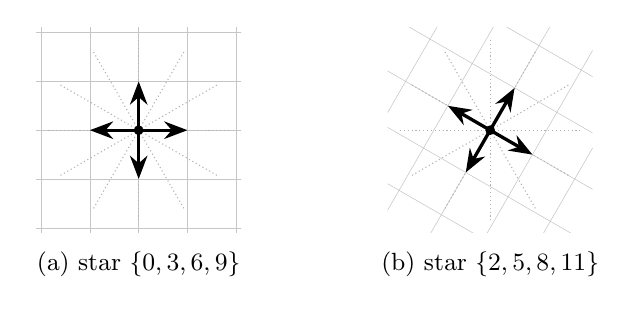
\begin{tikzpicture}[scale=0.62]
\begin{scope}
  \clip (-2.1,-2.1) rectangle (2.1,2.1);
  \draw[gray!45, very thin] (-3,-3) grid (3,3);
\end{scope}
\foreach \k in {0,...,11} \draw[gray!60, densely dotted] (0,0) -- (30*\k:1.9);
\foreach \k in {0,3,6,9} \draw[very thick, -{Stealth}] (0,0) -- (30*\k:1);
\fill (0,0) circle (2.8pt);
\node[font=\small] at (0,-2.75) {(a) star $\{0,3,6,9\}$};
\begin{scope}[xshift=7.2cm]
 \begin{scope}
  \clip (-2.1,-2.1) rectangle (2.1,2.1);
  \begin{scope}[rotate=60] \draw[gray!45, very thin] (-5,-5) grid (5,5); \end{scope}
 \end{scope}
 \foreach \k in {0,...,11} \draw[gray!60, densely dotted] (0,0) -- (30*\k:1.9);
 \foreach \k in {2,5,8,11} \draw[very thick, -{Stealth}] (0,0) -- (30*\k:1);
 \fill (0,0) circle (2.8pt);
 \node[font=\small] at (0,-2.75) {(b) star $\{2,5,8,11\}$};
\end{scope}
\end{tikzpicture}
\caption{Orientation selection for the square tiling: (a) the input frame, (b) the
canonical frame. Dotted rays mark the twelve directions $\omega^0,\dots,\omega^{11}$
(counterclockwise from $\omega^0$ on the right); thick arrows mark the occupied directions
of the origin's star. The word order prefers stars avoiding low direction indices, so the
canonical frame is the input rotated by $\omega^2$.}
\label{fig:square}
\end{figure}

\begin{figure}[t]
\centering
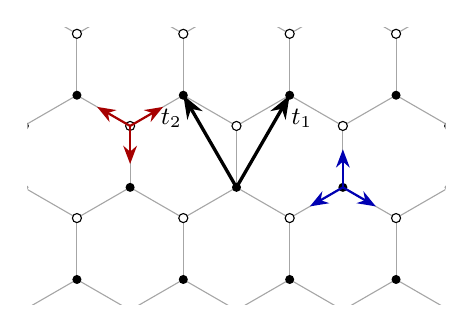
\begin{tikzpicture}[scale=0.78]
\begin{scope}
\clip (-3.4,-1.9) rectangle (3.4,2.6);
\foreach \i in {-3,...,3} \foreach \j in {-3,...,3} {
  \pgfmathsetmacro\ax{0.8660254*(\i-\j)}
  \pgfmathsetmacro\ay{1.5*(\i+\j)}
  \draw[gray!70] (\ax,\ay) -- ++(90:1);
  \draw[gray!70] (\ax,\ay) -- ++(210:1);
  \draw[gray!70] (\ax,\ay) -- ++(330:1);
}
\foreach \i in {-3,...,3} \foreach \j in {-3,...,3} {
  \pgfmathsetmacro\ax{0.8660254*(\i-\j)}
  \pgfmathsetmacro\ay{1.5*(\i+\j)}
  \fill (\ax,\ay) circle (2.1pt);
  \draw[fill=white] (\ax,\ay+1) circle (2.1pt);
}
\end{scope}
\draw[very thick, -{Stealth}] (0,0) -- (0.8660254,1.5) node[pos=0.75, right=1.5pt, font=\small] {$t_1$};
\draw[very thick, -{Stealth}] (0,0) -- (-0.8660254,1.5) node[pos=0.75, left=1.5pt, font=\small] {$t_2$};
\foreach \a in {90,210,330} \draw[thick, blue!70!black, -{Stealth}] (1.7320508,0) -- ++(\a:0.62);
\foreach \a in {30,150,270} \draw[thick, red!65!black, -{Stealth}] (-1.7320508,1) -- ++(\a:0.62);
\end{tikzpicture}
\caption{The honeycomb and its symbol data. Filled and open dots are the two vertex
classes; $t_1=\omega+\omega^3$ and $t_2=\omega^5+\omega^3$ span the period lattice. The
star of the filled class, drawn at a representative vertex on the right, is $\{3,7,11\}$;
the star of the open class, drawn on the left, is $\{1,5,9\}$. The word order picks the
filled class as the anchor in the canonical frame.}
\label{fig:honey}
\end{figure}

\section{Adversarial verification}\label{sec:verification}

Beyond the proofs, the reference implementation was subjected to an adversarial campaign;
all artifacts accompany this note.

\begin{itemize}\itemsep2pt
\item \emph{Differential against the baseline.} On a corpus of 290 symbols (the five
tilings of Table~\ref{tab:instances}; re-encodings across all four ambiguity sources
simultaneously; sublattice re-encodings of index 2, 4 and 6; single-edit mutants; 60 random
symbols with three scrambles each), $\N$ induces the byte-identical equivalence partition
(69 classes) as an independent implementation of the $24n$-frame baseline equipped with the
same Stage A. The two forms select different representatives, so partition agreement is the
meaningful comparison.
\item \emph{Frame lemma at full strength.} Lemma~\ref{lem:frame} was checked exhaustively,
not only at minima: for six symbols (including a chiral constellation, an all-empty-star
cloud, and a degenerate lattice with $\R$-dependent generators), all $24$ values of $h$,
three translations $c$, all $24$ values of $g'$ and every origin, about $5\times10^4$
matrix comparisons, zero violations. The $D_{12}$ composition table and the homomorphism
property of $\sigma$ were verified on all $576$ pairs.
\item \emph{Targeted adversaries.} A symbol whose star multiset is invariant under a strict
supergroup of its point group (so the residual minimization must compare genuinely distinct
candidates: $|\Gmin|=2$, two distinct candidates) and an empty-star cloud with trivial
point group ($|\Gmin|=24$, four anchors, 96 distinct candidates) were both stable under 300
random re-encodings; a chiral constellation and its explicit mirror image merge, as
\eqref{eq:equiv} requires. In total, canonicity was exercised on roughly $10^4$ randomized
re-encodings, including 131 of 400 random symbols whose ties required real tie-breaking.
\item \emph{Idempotence and Stage A.} $\N(\N(M))=\N(M)$ on the entire corpus; Stage A
recovered maximal lattices from re-encodings at indices up to 49 and leaves already-maximal
symbols unchanged; the rank-2 assertion of Lemma~\ref{lem:stagea}(d) never fired on 3000
random symbols.
\end{itemize}

Degenerate inputs are handled as follows: symbols violating the encoding contract (rank-1
lattices, empty seed lists) are rejected by assertion rather than canonicalized;
$\R$-linearly dependent lattice generators are accepted silently and canonicalized
consistently (the theory never uses $\R$-independence), which is acceptable for a dedup key
but callers wanting validation must test $\mathrm{Im}(t_1\overline{t_2})\neq0$ themselves.

\section{Limitations and open directions}\label{sec:limits}

\paragraph{T1 (directness).} What is proved: the frame search is cut from $24n$ to the
stabilizer $\sigma a$ of the star data by a direct, minimization-free rule, and internal
ties coming from true symmetries are provably redundant (Lemma~\ref{lem:ties}). What is not
proved: that refined equivariant invariants always pin a unique frame per symmetry orbit.
The residual minimization therefore remains as a correctness guarantee, and on symmetric
tilings it demonstrably compares only copies of one matrix. We do not claim
$\sigma a=O(1)$ generically over any natural distribution of tilings; the uniform tilings
of Table~\ref{tab:instances} all have $\sigma>1$, tracking their point groups.

\paragraph{T2 (entry bounds).} As delivered, $\N$ has no intrinsic entry bound: $\rep$
reduces pivot columns only, so free-column entries are bounded polynomially in the input
encoding but not by tiling data. A variant replaces the HNF basis by the Lagrange--Gauss
reduced basis (unique up to at most 16 ordered sign/swap/tie choices, realized on hexagonal
lattices; take the lexicographic minimum over them) and reduces seeds into the fundamental
parallelogram. Sketch of the resulting bound: each $\omega^k$ has coordinates in
$\{-1,0,1\}$, so a vertex reachable from the origin by $m$ unit-edge steps has all four
coordinates bounded by $m$ in absolute value; reduced representatives lie within Euclidean
distance $O(\lambda_2)$ of the origin, and $\lambda_2=O(n)$ since the cell area is
$\Theta(n)$ and $\lambda_1$ is bounded below by the minimum vertex distance of unit-edge
tilings. The missing step is the routine bounded-dilation lemma converting Euclidean
distance to path length in these tilings; we flag it rather than claim it. Conversely
$O(\sqrt n)$ is impossible: strip-stacked tilings in the style of the elongated triangular
family realize $\lambda_1=\Theta(1)$, $\lambda_2=\Theta(n)$, and any symbol must contain a
basis vector of length $\Theta(n)$, forcing entries $\Omega(n)$.

\paragraph{T3 (hardness).} Nothing is proved. We note only that once a frame $(g,o)$ is
fixed, the labeled structure is rigid: a breadth-first traversal of the quotient graph with
direction-sorted edges reconstructs the symbol deterministically in $O(n)$ operations, so
no canonical-labeling hardness can hide inside a frame. The entire search space of the
problem is the $24n$ frame set, already cut to the star stabilizer; a hardness reduction
would need families of tilings whose equivariant local invariants all coincide across
inequivalent frames, which the rigidity of the fifteen vertex types makes implausible, but
that is an expectation, not a theorem.

\paragraph{Relation to prior sketches.} Anchoring the origin at an extremal intrinsic label
and fixing the orientation by star minimization realizes, with proofs, the dual-graph
canonical-labeling sketch of~\cite[\S5.10]{soto2020thesis}; the contributions here are the
equivariance framework making the restricted minimum well defined, the coincidence lemma,
and the lattice-maximality correction of Remark~\ref{rem:gap}.

\begin{thebibliography}{9}
\bibitem{soto2021integer}
J.~E. Soto S\'anchez, T.~Weyrich, A.~Medeiros~e~S\'a, L.~H. de~Figueiredo,
\emph{An integer representation for periodic tilings of the plane by regular polygons},
Computers \& Graphics 95 (2021) 69--80.

\bibitem{soto2020thesis}
J.~E. Soto S\'anchez,
\emph{On Periodic Tilings with Regular Polygons},
PhD thesis, IMPA, 2020.

\bibitem{cohen1993}
H.~Cohen,
\emph{A Course in Computational Algebraic Number Theory},
Graduate Texts in Mathematics 138, Springer, 1993.

\bibitem{grunbaum1987}
B.~Gr\"unbaum, G.~C. Shephard,
\emph{Tilings and Patterns},
W.~H. Freeman, 1987.
\end{thebibliography}

\end{document}
